% !TeX root = ../apuntes-ea.tex

\chapter{Biyecciones}

\section{El por qué de la notación cíclica}

\begin{dfn}
	Sea $X$ un conjunto. Definimos
	\begin{align*}
		\biy{X} = \{f: X \to X \mid f \text{ es biyección}\}
	\end{align*}
\end{dfn}

Como coinciden dominio y codominio ($f:X \to X$) si $f$ es inyectiva entonces automáticamente es sobre y por tanto biyectiva.

En general, tiene sentido pensar en $Biy(X)$ aunque $|X| = \infty$. Además, en dicho conjunto viven la biyección identidad y la biyección inversa para cada biyección. Por tanto, tiene sentido pensar en $(Biy(X), \circ)$ como un grupo (la composición de biyecciones da una biyección). Lo escribimos en forma de teorema.

\begin{thm}
	Sea $X$ un conjunto. El par $(\biy{X}, \circ)$ es un grupo.
\end{thm}

Nos concentraremos en el caso en el que $|X| = n < \infty$ que nos da $Biy(X) = S_n$. Ver \autoref{dfn:sn} para una explicación detallada del grupo $S_n$.

Fijamos un conjunto $X$ y un homomorfismo de grupos $\alpha: X \to Biy(X)$. A partir de estos datos definimos una relación de equivalencia que nos da una partición de $X$, es decir, vamos a partir $X$ en conjuntos disjuntos. Veamos un ejemplo particular.

\begin{ej}
	Supongamos $G = X,\ |G| = n$ y consideramos $\rho: G \to \autom{G} \subset Biy(X)$. Definimos la relación en $X = G$
	\begin{align*}
	aRb \iff \exists g \in G \mid \phi_g(a) = b,\ \phi_g(x) = gx\inv{g}
	\end{align*}
	que es la relación de conjugación dada por el isomorfismo de conjugación de toda la vida.
	
	Ahora, en lugar de pensar en $G = X$ pensamos en $X = \{H < G\}$ (los subgrupos de $G$). Para cualquier isomorfismo de grupos $\beta: G \to G$, tenemos que si $H < G$ entonces $\beta(H) < G$.
	
	Lo que hemos hecho aquí es un caso particular de lo que viene ahora.
\end{ej}

Ahora pasamos al caso general.

\begin{pro}
	Sea $\alpha: G \to Biy(X),\ g \mapsto \alpha(g)$ un homomorfismo de grupos\footnote{Ojo: aquí las imágenes de los elementos $g \in G$ son biyecciones $f:G \to G$, por eso tendrá sentido la notación $\alpha(g)(a)$ que significa aplicar la función que nos devuelve $\alpha$ al elemento $a \in G$.}. Definimos la relación de equivalencia $R$ en el conjunto $X$
	\begin{align}
	aRb \iff \exists g \in G \mid \alpha(g)(a) = b
	\end{align}
	Afirmamos que la relación es de equivalencia y que nos divide $X$ en subconjuntos disjuntos (nos particiona $X$).
\end{pro}

\begin{proof}Probamos las 3 propiedades de las relaciones de equivalencia.
	\begin{enumerate}
		\item Reflexiva: $\forall x \in X, a R a$. Por ser $\alpha$ homomorfismo tenemos que $\alpha(e_G) = id_X$ y por tanto $\alpha(e_G)(a) = a$.
		\item Simétrica: $aRb \implies bRa$. Partimos de que $\exists g \in G \mid \alpha(g)(a) = b$. Tomamos $\inv{g} \in G$ y por ser $\alpha$ homomorfismo de grupos tenemos que $\alpha(\inv{g})(b) = \inv{(\alpha(g))}(b) = a$.
		\item Transitiva: $aRb \land bRc \implies aRc$. Partimos de que $\exists g, g' \in G \mid \alpha(g)(a) = b \land \alpha(g')(b) = c$. Tomamos $g'g \in C$ y tenemos que $\alpha(g'g)(a) = \alpha(g')(\alpha(g)(a)) = \alpha(g')(b) = c$ por composición de biyecciones.
	\end{enumerate}
\end{proof}

¿Cómo son las clases que da la partición?

Pues tenemos que para $a \in X$, la clase $cl(a) = \{\alpha(g)(a) \mid g \in G\}$. Definimos $H_a = \{g \in G \mid \alpha(g)(a) = a\}$. Tenemos por lo visto anteriormente que $H_a < G \land |cl(a)| = [G:H_a]$. Entonces tenemos lo siguiente:
\begin{itemize}
	\item En el caso en que $X = G$, es decir, que el conjunto $X$ tiene dentro \textit{elementos} de $G$, tenemos que $H_a = C(a)$ donde $C(a)$ es el centralizador de $a$ (\autoref{dfn:centralizador}).
	\item En el caso en que $X = \{H < G\}$, es decir, que el conjunto $X$ tiene dentro \textit{subgrupos} de $G$, tenemos que $H_a = N(a)$ donde $N(a)$ es el normalizador de $a$ (\autoref{dfn:normalizador}).
\end{itemize}

Vista la definición abstracta, lo que nos interesa de esto es aplicarlo a los grupos $S_n$ de los que hablábamos antes. En particular, ahora daremos una definición formal de ciclo para la notación que introdujimos en la \autoref{sec:notacionciclica}.

\begin{wrapfigure}{l}{0.3\textwidth}
	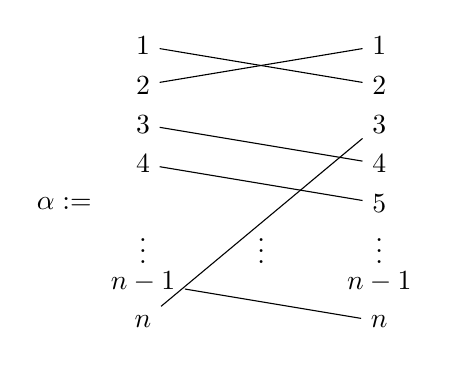
\begin{tikzpicture}
	\begin{scope}[scale=0.5]
	\node (alpha) at (-2, 0) {$\alpha :=$};
	\node (1) at (0,4) {$1$};
	\node (2) at (0,3) {$2$};
	\node (3) at (0,2) {$3$};
	\node (4) at (0,1) {$4$};
	\node (dots) at (0,-1) {$\vdots$};
	\node (nmenos1) at (0,-2) {$n-1$};
	\node (n) at (0,-3) {$n$};
	
	\node (1p) at (6,4) {$1$};
	\node (2p) at (6,3) {$2$};
	\node (3p) at (6,2) {$3$};
	\node (4p) at (6,1) {$4$};
	\node (5p) at (6,0) {$5$};
	\node (dotsp) at (6,-1) {$\vdots$};
	\node (nmenos1p) at (6,-2) {$n-1$};
	\node (np) at (6,-3) {$n$};
	
	\node (dotsc) at (3, -1) {$\vdots$};
	
	
	\draw (1) -- (2p);
	\draw (2) -- (1p);
	\draw (3) -- (4p);
	\draw (4) -- (5p);
	\draw (nmenos1) -- (np);
	\draw (n) -- (3p);
	\end{scope}
	\end{tikzpicture}
	\caption{La permutación $\alpha$ de $S_n$}
	\label{fig:permalphaejpart}
\end{wrapfigure}

Fijamos $\sigma \in S_n$ y definimos $G = \gen{\sigma}$ el subgrupo generado por $\sigma$ en $S_n$. Definimos ahora el homomorfismo
\begin{align*}
G = \gen{\sigma} & \to S_n = \biy{X},\qquad X = \{1, 2, 3, \dots, n\}
\end{align*}
Las clases $cl(i)$ para $i \in \{1, 2, \dots, n\}$ son de la forma\footnote{Las clases serían de la forma $\alpha(g)(i)$ pero es que en este caso todos los $\alpha(g)$ son elementos de $G = \gen{\sigma}$ y por tanto son de la forma $\sigma^k$.}
\begin{align*}
cl(i) = \{\sigma^k(i) \mid k \in \Z\}
\end{align*}


\begin{ej}
	Consideramos la permutación $\alpha \in S_n$ dada por (ver \autoref{fig:permalphaejpart})
	\begin{align*}
		\alpha = \begin{array}{ccccccc}
		1 & 2 & 3 & 4 & \dots & n-1 & n \\
		2 & 1 & 4 & 5 & \dots & n & 3
		\end{array}
	\end{align*}
	que en la notación cíclica podríamos escribir como $\alpha = (345\dots n)(12)$.
	
	En este caso la clase $cl(1) = \{1, 2\} = cl(2)$ está formada por los elementos que podemos obtener de aplicar $\alpha$ al elemento $1$. Ya se intuye la utilidad de la notación cíclica: la permutación $\alpha$ nunca mezcla elementos de la caja $\{1,2\}$ con elementos de la caja $\{3, 4, 5, \dots, n\}$. Así, también tendremos que $cl(3) = cl(4) = \dots = cl(n) = \{3, 4, 5, \dots, n\}$. Los elementos que hay en estas dos clases coinciden con los elementos que hay en cada uno de los ciclos en los que hemos descompuesto $\alpha$.
\end{ej}

Vemos que si fijamos $\sigma$ se define una partición en $\{1, \dots, n\}$ de subconjuntos disjuntos
\begin{align*}
F_1 \cup F_2 \cup \dots \cup F_n
\end{align*}

Si $r = |F_i| > 1$, $F_i = \{i_0, i_1, \dots, i_r\}$ tal que $\sigma(i_0) = i_1, \sigma(i_1) = i_2, \dots, \sigma(i_r) = i_0$.

\begin{dfn}[Ciclo]
	\label{dfn:ciclo}
	Diremos que $\sigma$ es un ciclo de longitud $r$ si en la partición definida
	\begin{align*}
	F_1 \cup F_2 \cup \dots \cup F_n
	\end{align*}
	todas las cajas $F_j,\ j < r$ tienen un único elemento y $F_r$ tiene $r$ elementos.
\end{dfn}

La definición quiere decir que, en el fondo, un ciclo es un tipo de permutación que al aplicarla sucesivamente sobre el conjunto $X$ lo particiona en varias cajas pero de manera que todas tienen un elemento excepto una, que tiene todos los elementos que se mueven entre ellos por la acción del ciclo. Un ejemplo en el conjunto $X = \{1, 2, 3, \dots, n\}$ sería

\begin{center}
	\begin{tabular}{|c|c|c|c|}
		\hline
		1 & 5 & \dots & \vdots \\\cline{2-4}
		2 & 6 & $\ddots$ & \vdots \\\cline{2-4}
		3 & $\ddots$ & $\ddots$ & \vdots  \\\cline{2-4}
		4 & \dots & \dots & n\\\hline
	\end{tabular}
\end{center}

Observemos que por la notación que hemos elegido, los ciclos tienen la estructura $(\sigma^0(a)\ \sigma^1(a)\ \sigma^2(a) \dots \sigma^s(a))$ donde $\sigma$ es un elemento de $S_n$ y $a$ un elemento de $X$. Dado que si $\sigma^k = Id$ entonces $\sigma^{k + i} = \sigma^i$, si \textit{rotamos} los números que definen el ciclo no estamos haciendo nada. Esto es, el ciclo $(1234) = (2341) = (3412) = (4123)$.

\section{De permutaciones a composiciones de ciclos}

\begin{pro}
	Toda biyección $\alpha \in S_n$ se puede expresar como composición de ciclos disjuntos dos a dos:
	\begin{align*}
		\alpha = \sigma_1 \circ \sigma_2 \circ \dots \circ \sigma_s
	\end{align*}
\end{pro}

\begin{pro}
	La composición de dos ciclos disjuntos conmuta, es decir, si $\sigma_1$ y $\sigma_2$ son ciclos disjuntos (que no comparten ningún elemento entre los paréntesis) entonces $\sigma_1 \circ \sigma_2 = \sigma_2 \circ \sigma_1$
\end{pro}

\begin{cor}
	Toda descomposición de una permutación $\alpha \in S_n$ en ciclos disjuntos $\alpha = \sigma_s \circ \sigma_{s-1} \circ \dots \circ \sigma_2 \circ \sigma_1$ se puede reordenar sin cambiar el resultado.
\end{cor}

\begin{ej}
	Antes de seguir veamos un ejemplo más de cómo una biyección de $S_n$ particiona el conjunto $X = \{1, 2, \dots, n\}$.
	
	Consideramos $\alpha \in S_n$ definida con
	\begin{align*}
		\alpha = \left(\begin{array}{cccccccccc}
		1 & 2 & 3 & 4 & 5 & 6 & 7 & 8 & 9 & 10 \\
		2 & 3 & 1 & 5 & 6 & 4 & 7 & 9 & 8 & 10
		\end{array}\right)
	\end{align*}
	
	La partición que nos da $\alpha$ de $X = \{1, 2, 3, 4, 5, 6, 7, 8, 9 10\}$ es la siguiente:
	\begin{center}
		\begin{tabular}{|c|c|c|c|}
			\hline
			1 & 4 & 7 & \\ \cline{3-3}
			2 & 5 & 8 & 10 \\
			3 & 6 & 9 & \\
			\hline
		\end{tabular}
	
		Partición de $X$ dada por $\alpha = (123)(456)(89)$
	\end{center}
	Esto lo obtenemos de buscar las clases de cada elemento. Empezamos por el que queramos, por ejemplo, el $1$:
	\begin{align*}
		cl(1) = \{\alpha^k(1) \mid k \in \Z\} = \{\alpha^0(1) = 1, \alpha^1(1) = 2, \alpha^2(1) = 3, \alpha^3(1) = 1, \alpha^4(1) = 2, \dots \}
	\end{align*}
	Eliminando duplicidades obtenemos que $cl(1) = \{1,2,3\}$. Análogamente obtenemos $cl(4) = \{4,5,6\},\ cl(7) = \{7\},\ cl(8) = \{8,9\},\ cl(10) = \{10\}$. Lo que hemos hecho es seguir el algoritmo descrito en la \autoref{sec:notacionciclica}, esta vez entendiendo el significado. Obtenemos que $\alpha = (123)(456)(89)$ o cualquier reordenación de los ciclos anteriores, ya que al ser disjuntos, cambiar el orden en el que los rotamos no afecta al resultado.
\end{ej}

\begin{wrapfigure}{l}{0.3\textwidth}
	\centering
	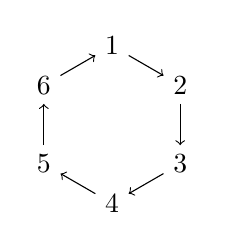
\begin{tikzpicture}
	\node (1) at (0,1) {${1}$};
	\node (2) at (0.866,0.5) {$2$};
	\node (3) at (0.866,-0.5) {$3$};
	\node (4) at (0, -1) {$4$};
	\node (5) at (-0.866, -0.5) {$5$};
	\node (6) at (-0.866,0.5) {$6$};
	
	\draw[->] 	(1) edge (2)
	(2) edge (3)
	(3) edge (4)
	(4) edge (5)
	(5) edge (6)
	(6) edge (1);
	\end{tikzpicture}
	\caption{El ciclo $\sigma = (123456)$}
	\label{fig:ciclo16}
	
	
	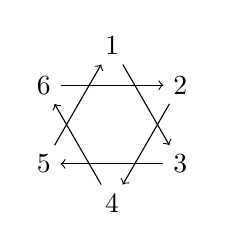
\begin{tikzpicture}
	\node (1) at (0,1) {${1}$};
	\node (2) at (0.866,0.5) {$2$};
	\node (3) at (0.866,-0.5) {$3$};
	\node (4) at (0, -1) {$4$};
	\node (5) at (-0.866, -0.5) {$5$};
	\node (6) at (-0.866,0.5) {$6$};
	
	\draw[->] 	(1) edge (3)
	(3) edge (5)
	(5) edge (1)
	(2) edge (4)
	(4) edge (6)
	(6) edge (2);
	\end{tikzpicture}
	\caption{El ciclo $\sigma^2 = (123456)^2$}
	\label{fig:ciclo16cuadrado}
	
	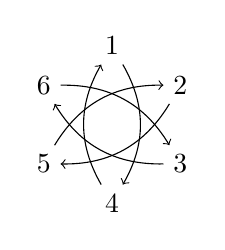
\begin{tikzpicture}
	\node (1) at (0,1) {${1}$};
	\node (2) at (0.866,0.5) {$2$};
	\node (3) at (0.866,-0.5) {$3$};
	\node (4) at (0, -1) {$4$};
	\node (5) at (-0.866, -0.5) {$5$};
	\node (6) at (-0.866,0.5) {$6$};
	
	\draw[->] 	(1) edge[bend left] (4)
	(4) edge[bend left] (1)
	(2) edge[bend left] (5)
	(5) edge[bend left] (2)
	(3) edge[bend left] (6)
	(6) edge[bend left] (3);
	\end{tikzpicture}
	\caption{El ciclo $\sigma^3 = (123456)^3$}
	\label{fig:ciclo16cubo}
\end{wrapfigure}

Veamos ahora cómo se relacionan los órdenes de los ciclos con su longitud.


\begin{ej}
	Consideramos $\sigma = (123456) \in \S_n$. Observamos que $\sigma^6 = Id$ es decir que $\sigma$ tiene orden 6.
	
	De esta manera si nos preguntan por $\sigma^{122} = (123456)^{122} = (123456)^{6\cdot20} \circ (123456)^2 = (123456)^2$ no nos asustamos.
	
	Si nos hubieran dado $\sigma$ con la notación habitual, aparte de que hubiera ocupado mucho, no podríamos haber resuelto esta operación tan rápido.
\end{ej}


\begin{ej}
	Nos preguntamos ahora por las potencias de $\sigma = (123456)$ menores que $6 = o(\sigma)$.
	\begin{itemize}
		\item $\sigma^2$ equivaldría a aplicar $\sigma$ dos veces a cada número $\{1, \dots, 6\}$ (los demás números no nos interesan porque sabemos que $\sigma$ no los mueve). Ayudándonos del dibujo obtenemos que $\sigma^2 = (135)(246)$.
		
		Se verifica que $\sigma^2$ tiene $o(\sigma^2) = 3$ y además si recordamos el \autoref{thm:ordendepotencia} comprobamos que se verifica $o(\sigma^2) = \frac{o(\sigma)}{mcd(o(\sigma), 2)} = \frac{6}{2} = 3$.
		
		\item En cuanto a $\sigma^3$ observamos que al aplicar $\sigma$ 3 veces nos quedan 3 ciclos y que se vuelve a verificar que $o(\sigma^3) =\frac{o(\sigma)}{mcd(o(\sigma), 3)} = \frac{6}{3} = 2$
	\end{itemize}
\end{ej}

Esto nos lleva a enunciar el siguiente teorema

\begin{thm}
	\label{thm:ordenpotenciasciclos}
	Sea $\sigma = (i_1\ i_2\ i_3 \dots i_n)$ un ciclo de longitud $n$. Sea $m \in \Z$ y $d = mcd(n,m)$. Entonces $\sigma^m$ es un producto de $d$ ciclos de longitud $\frac{n}{d}$ y estos son disjuntos dos a dos.
\end{thm}

Poder averiguar los órdenes de ciclos es una herramienta muy potente. Por ejemplo, podemos hacer lo siguiente.

\begin{ex}[H3.8]
	Demuestra que el subgrupo $G < S_4$ generado por los elementos $\sigma = (1432)$ y $\tau = (24)$ es isomorfo a $D_4$.
\end{ex}

\begin{proof}
	Sabemos que $o(\sigma) = 4$ y que $o(\tau) = 2$. Trabajando un poco vemos que
	\begin{align*}
		\gen{\sigma} &= \{\sigma = (1432), \sigma^2 = (13)(24), \sigma^3 = (4321), \sigma^4 = Id\} \\
		\gen{\tau} &= \{\tau = (24), \tau^2 = Id\}
	\end{align*}
	Faltaría ver que $\sigma \tau = \tau \sigma^3$ es decir que $(1432)(24) = (24)(4321)$ (spoiler: es verdad) y ya podríamos identificar $\sigma$ con $B$ y $\tau$ con $A$ para obtener la presentación del famoso grupo $D_4$:
	\begin{align*}
		D_4 \isom G = \gen{\sigma, \tau \mid o(\sigma) = 4 \land o(\tau) = 2 \land \sigma \tau = \tau \sigma^3}
	\end{align*}
\end{proof}

\begin{thm}
	Sea $\alpha$ una permutación expresada como composición de ciclos disjuntos $\alpha = \sigma_1 \circ \sigma_2 \circ \dots \circ \sigma_n$. Entonces el orden de $\alpha$ es el mínimo común múltiplo de los órdenes de cada $\sigma_i$:
	\begin{align*}
		\alpha = \sigma_1 \circ \sigma_2 \circ \dots \circ \sigma_n \text{ disjuntos } \implies o(\alpha) = mcm(\sigma_1, \dots, \sigma_n)
	\end{align*}
\end{thm}

% TODO demostrar esto: dorronsoro página 120

\begin{proof}
	Ver \cite{dor96} página 120.
\end{proof}

\section{Trasposiciones}

\begin{dfn}[Trasposición]
	Una trasposición es un ciclo de orden 2. Cualquier trasposición tiene orden 2.
\end{dfn}

Las trasposiciones tienen la forma $(a\ b)$ pero observemos que también se pueden escribir como $(b\ a)$ ya que lo que estamos haciendo es \textit{rotar} (o empezar en otro lugar del ciclo).

\begin{pro}
	La inversa de cualquier trasposición es ella misma.
\end{pro}

\begin{thm}
	El grupo $S_n$ está generado por las transposiciones $\sigma \in S_n$.
\end{thm}

Ya sabemos que cualquier permutación se puede expresar como producto de ciclos [disjuntos]. Para probar este teorema probaremos la siguiente proposición:

\begin{pro}
	Cualquier ciclo se puede expresar como composición de trasposiciones.
\end{pro}

La prueba es constructiva y describe la manera de expresar un ciclo como composición de trasposiciones.

\begin{proof}
	Sabemos que un ciclo $\sigma$ se escribe como $\sigma = (\sigma^0(a) = a\ \sigma^1(a)\ \sigma^2(a)\ \dots \ \sigma^s(a))$. Pues vasta con observar que la composición
	\begin{align*}
		\sigma = (a\ \sigma^s(a))(a\ \sigma^{s-1}(a))\dots(a\ \sigma^2(a))(a\ \sigma(a))
	\end{align*}
	tiene el mismo efecto.
\end{proof}

\begin{ej}
	La permutación $\sigma = (1234)$ se puede expresar como $\sigma = (14)(13)(12)$.
\end{ej}

\subsection{Paridad de las trasposiciones}

\begin{thm}
	\label{thm:paridadpermutaciones}
	Si $\sigma \in S_n$ se puede descomponer como un número par de trasposiciones entonces toda expresión en $\sigma$ expresada como una composición de un número par de trasposiciones.
	
	Análogamente para las permutaciones que se pueden expresar como una composición de un número impar de trasposiciones.
\end{thm}

\begin{proof}
	Definimos una función
	\begin{align*}
		S_n &\to GL_n(\N)\\
		\sigma &\mapsto \left(\begin{array}{ccc}
		e_\sigma(1) & \dots & e_\sigma(n) \\
		\vdots & \vdots & \vdots
		\end{array}\right)
	\end{align*}
	Esta función es un homomorfismo de grupos.
	
	Entonces si expresamos $\sigma$ como composición de trasposiciones $\sigma = (i_1^{(1)}\ i_2^{(1)})(i_1^{(2)}\ i_2^{(2)}) \dots (i_1^{(r)}\ i_2^{(r)})$ y aplicamos la función que hemos definido nos queda
	\begin{align*}
		A = \left(\begin{array}{ccc}
		e_\sigma(1) & \dots & e_\sigma(n) \\
		\vdots & \vdots & \vdots
		\end{array}\right) = \underbrace{\left(\begin{array}{ccc}
			i_1^{(1)} & \dots & i_2^{(1)} \\
			\vdots & \vdots & \vdots
			\end{array}\right)}_{\det = -1} \dots \underbrace{\left(\begin{array}{ccc}
			i_1^{(r)} & \dots & i_2^{(r)} \\
			\vdots & \vdots & \vdots
			\end{array}\right)}_{\det = -1}
	\end{align*}
	y entonces
	\begin{align*}
		\det A = (-1)^r = \begin{cases}
		1 &\text{ si r es par} \\
		-1 &\text{ si r es impar}
		\end{cases}
	\end{align*}
\end{proof}

Visto que la paridad de una permutación va a ser invariante por la expresión como composición de trasposiciones que elijamos vamos a darle nombre ya que parece importante

\begin{dfn}[Paridad de una permutación]
	Sea $\sigma \in S_n$.
	\begin{itemize}
		\item Diremos que $\sigma$ es par si se puede descomponer como una composición de un número par de trasposiciones.
		
		\item Diremos que $\sigma$ es impar si se puede descomponer como una composición de un número impar de trasposiciones.
	\end{itemize}
\end{dfn}

En otros textos, esto se define con la \textit{signatura}

\begin{dfn}[Signatura de una permutación]
	Sea $\sigma \in S_n$ una permutación que podemos descomponer como una composición de $r$ trasposiciones: $\sigma = \tau_1 \circ \tau_2 \circ \dots \circ \tau_r$. Llamamos signatura de $\sigma$ al número $(-1)^r$ y lo denotamos por $\text{sig}(\sigma) = (-1)^r$.
\end{dfn}

Es muy interesante la manera en la que hemos demostrado el \autoref{thm:paridadpermutaciones}. El homomorfismo que hemos construido de $S_n$ a $GL_n(\N)$ se puede extender para llegar al determinante:

\begin{align*}
	\varphi : S_n &\to GL_n(\R) &\to (\{-1, 1\}, \cdot) \\
	\sigma &\mapsto A = \left(\begin{array}{ccc}
	e_\sigma(1) & \dots & e_\sigma(n) \\
	\vdots & \vdots & \vdots
	\end{array}\right) &\mapsto \det(A)
\end{align*}

Si consideramos el homomorfismo desde $S_n$ hasta $(\{-1, 1\}, \cdot)$ nos damos cuenta de que hemos definido un homomorfismo de grupos que además es sobreyectivo.

El núcleo de dicho isomorfismo $\ker \varphi = \{\sigma \in S_n \mid \varphi(\sigma) = 1\}$ es un subgrupo por el teorema de correspondencia entre familias de subgrupos bajo un epimorfismo (ver \autoref{thm:correspondenciasubgruposdor96}). Además este subgrupo es normal y de índice 2. Tan importante es que le damos nombre.

\begin{dfn}[Grupo alternado]
	Sea $\varphi: S_n \to ({-1, 1}, \cdot)$ el homomorfismo de grupos definido arriba. Definimos el grupo alternado $A_n$ como
	\begin{align*}
		A_n = \ker \varphi = \{\sigma \in S_n \mid \sigma \text{ es par}\}
	\end{align*}
\end{dfn}

Recogemos los resultados que hemos dejado caer antes de la definición:

\begin{pro}
	$A_n \normsub S_n$ y además $[S_n : A_n] = 2$
\end{pro}

\begin{cor}
	Todo grupo $S_n$ tiene un subgrupo normal de orden $2$.
\end{cor}